\documentclass[../chapter-2-spline-representation.tex]{subfiles}
\begin{document}
\subsubsection{The limiting behaviour of $H_\lambda$}


The inspection of the hat matrix 

\[
H_\lambda = W B\left(W B^\prime W B +  \lambda_l P_l + \lambda_m P_m \right)^{-1} \left(W B\right)^\prime D^{-1}.
\]
\noindent
and its properties are integral for assessing model complexity and selecting the optimal values of the tuning parameters $\lambda_l$ and $\lambda_m.$  Summarizing the complexity of a fitted P-spline is far from a trivial task; one must simultaneously consider the value of the smoothing parameter, the number of basis functions in the B-spline basis, as well as the order of the difference penalties. We follow \citet{eilers1996flexible} and\citet{marx2005multidimensional} assess model complexity as discussed in cite{hastie1990generalized}, who proposed to use the trace of the smoother matrix as an approximation  to the effective dimensions of linear smoother. The \emph{effective dimension} is easily obtained and combines the effect of all three of these elements: 

%This approach to approximating the effective model dimension is also consistent with \citet{ye1998measuring}, who constructed a generalization of the concept of a model's degrees of freedom using the idea that the degrees of freedom can also be interpreted as the sum of the sensitivity of each fitted value with respect to the corresponding observed value.  For smoothing matrix $H$, the predicted response values are given by $\hat{y} = H y$. Writing
%
%\begin{align*}
%\frac{\partial \hat{y_i}}{\partial y_i} = \frac{\partial }{\partial y_i} \sum_{j} h_{ij} y_j = h_{ii},
%\end{align*}
%\noindent
%we see that the latter interpretation of the effective model dimension reduces to calculating the trace of the hat matrix. Thus we take the effective dimension to be 
%\begin{align}
%\textup{ED}\left(\lambda\right) &= \textup{tr}\left(H\right) \nonumber \\
%&= \textup{tr}\bigg[ B\left( B^T B + \lambda D^T D \right)^{-1} B^T\bigg], \label{eq:hat_matrix_trace}
%\end{align}

\begin{align}
\begin{split} \label{eq:hat-matrix-trace}
\textup{ED} &= \textup{tr} \left[ H_\lambda \right]\\
&= \textup{tr}\bigg[\left[WB \left(WB\right)^\prime D^{-1}WB +  \lambda_l P_l+ \lambda_m P_m\right]^{-1} \left(W B\right)^\prime D^{-1}  \bigg]
\end{split}
\end{align}
\noindent
When the number of basis functions is significantly smaller than the sample size, it is computationally advantageous to use the cyclic property of the trace: 

\begin{equation*}
\textup{tr}\bigg[\left[ \left(WB\right)^\prime D^{-1}WB +  \lambda_l P_l+ \lambda_m P_m\right]^{-1} \left(W B\right)^\prime D^{-1} WB  \bigg],
\end{equation*}
\noindent
which requires computing the trace of a $KL \times KL$ matrix. The effective dimension approaches $d_l + d_m$, the order of the differencing operator, as $\lambda$ increases, where $d_l$ and $d_m$ denote the orders of the difference penalties in the $l$ and $m$ directions, respectively.  Let
\begin{equation*}
Q = \left(W B\right)^\prime D^{-1} WB \qquad \mbox{and} \qquad Q_\lambda = P.
\end{equation*}

Using properties of the matrix trace, we can write
\begin{align*}
%\begin{split}
\mbox{tr}\left(H_\lambda \right) &= \mbox{tr}\bigg[ \left(Q + Q_\lambda \right)^{-1}Q \bigg]\\
&=\mbox{tr}\bigg[ Q^{1/2}\left(Q + Q_\lambda \right)^{-1}Q^{1/2} \bigg] \\
&=\mbox{tr}\bigg[\left(I + Q^{-{1/2}}Q_\lambda Q^{-{1/2}} \right)^{-1} \bigg]
%\end{split}
\end{align*}
Define $L \equiv Q^{-{1/2}}Q_\lambda Q^{-{1/2}}$. Then
\begin{equation*}
\mbox{tr}\left(H_\lambda \right) = \mbox{tr}\bigg[\left(I + \lambda L \right)^{-1} \bigg] = \sum_{j=1}^n \frac{1}{1 + \lambda \gamma_j}
\end{equation*}
 where $\gamma_j$, $j=1,\dots,n$ are the eigenvalues of $L$. $Q_\lambda$ has exactly $d_l + d_m$ eigenvalues equal to zero. Hence, $L$ has $d_l + d_m$ zero eigenvalues. For large $\lambda$, only the $d_l + d_m$ terms with $\gamma_j=0$ contribute to the sum which gives the trace of $H$, so that
 \[
\lim_{\lambda \rightarrow \infty  } \mbox{tr}\left(H\right) = d_l + d_m.
 \]

%A further simplification of \ref{eq:hat-matrix-trace}
%
%\begin{align*} 
%\left(B^T B + \lambda D^T D \right)^{-1} B^T B &= \left(B^T B + \lambda D^T D \right)^{-1} \left( B^T B + \lambda D^T D - \lambda D^T D\right) \nonumber \\
%&= I - \lambda\left(B^T B + \lambda D^T D \right)^{-1} D^T D \label{eq:cyclic_hat_matrix_simplification}
%\end{align*}
%
%\begin{align*} 
%\left[\left(WB\right)^\prime D^{-1}WB +  \lambda_l P_l+ \lambda_m P_m\right]^{-1} \left(W B \right)^\prime D^{-1} WB  &= \left[\left(WB\right)^\prime D^{-1}WB +  \lambda_l P_l+ \lambda_m P_m\right]^{-1}\left(W B \right)^\prime D^{-1} \times \\
%&\mbox{\;\;\;\;\;\;\;\;\;\;\;\;\;\;\;\;\;\;\;\;\;} \left[WB + \lambda_l P_l+ \lambda_m P_m - \left(\lambda_l P_l+ \lambda_m P_m\right) \right] \\
%&= I - \lambda\left(B^T B + \lambda D^T D \right)^{-1} D^T D \label{eq:cyclic_hat_matrix_simplification}
%\end{align*}

Equation~\ref{eq:cyclic_hat_matrix_simplification} cleanly shows that the effective dimension is always less than $n$, the number of B-spline used in the regression basis; further, the effective dimension is always smaller than $\min\left(m,n\right)$. A formal proof follows below. This is illustrated in 

Figure~\ref{fig:PS_ED_figure_1} shows how the effective dimension on a univariate P-spline changes with the smoothing parameter for the ten simulated observations in Figure~\ref{fig:overcomplete_basis_pspline} using 60 B-spline basis functions. For small $\lambda$, the effective dimension approaches $m$. As $\lambda$ increases, the effective dimension approaches the order of the difference penalty, $d$. It is worth pointing out here that there are no problems incurred when smoothing with many more B-splines than observations since the effective model dimension is always less than $m$, for all $\lambda$. 

%\begin{figure}[H]
%\begin{subfigure}{.5\textwidth}
%  \centering
%   \graphicspath{{img/}}
%  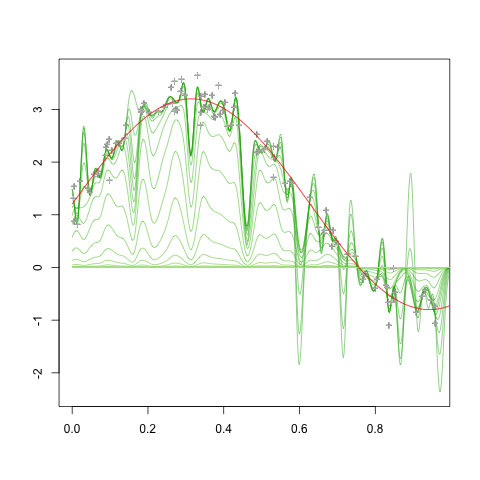
\includegraphics[scale=0.5]{PS_penalty_section_figure_6_order_0.png}
%  %\label{fig:pspline_small_lambda}
%\caption{$d=0$ }
%\end{subfigure}
%\begin{subfigure}{.5\textwidth}
%  \centering
%   \graphicspath{{img/}}
%  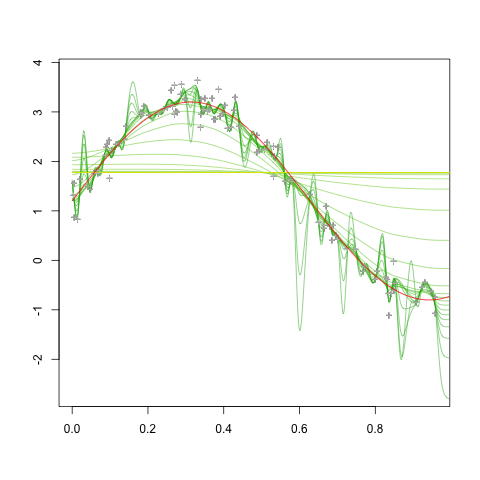
\includegraphics[scale=0.5]{PS_penalty_section_figure_6_order_1.png}
% % \label{fig:pspline_small_lambda}
%\caption{$d=1$}
%\end{subfigure}
%\begin{subfigure}{.5\textwidth}
%  \centering
%   \graphicspath{{img/}}
%  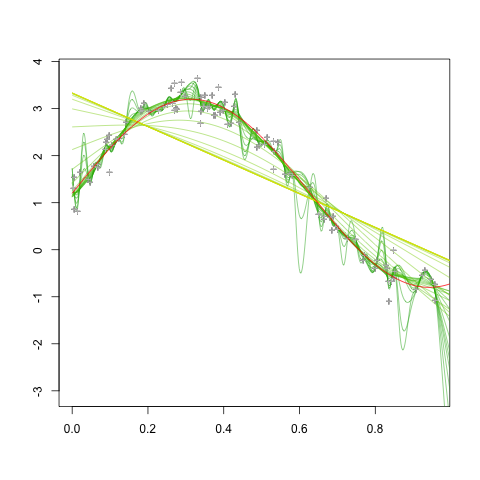
\includegraphics[scale=0.5]{PS_penalty_section_figure_6_order_2.png}
%  %\label{fig:pspline_small_lambda}
%\caption{$d=2$}
%\end{subfigure}
%\begin{subfigure}{.5\textwidth}
%  \centering
%   \graphicspath{{img/}}
%  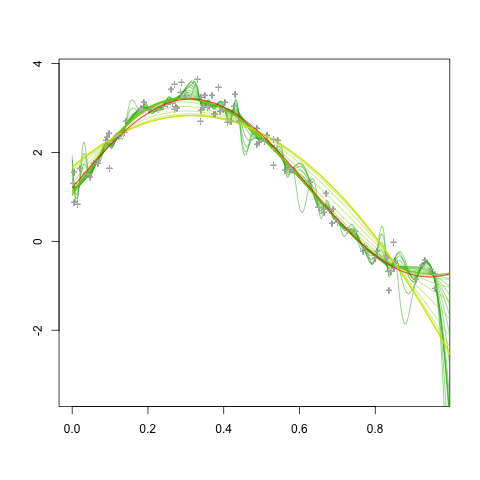
\includegraphics[scale=0.5]{PS_penalty_section_figure_6_order_3.png}
%  %\label{fig:pspline_small_lambda}
%\caption{$d=3$}
%\end{subfigure}
%\caption{\textit{Illustration of the impact of the order of the difference penalty. The number of B-splines used is the same in each plot, with the penalty parameter varying from across the same grid of values. The fitted curves in the upper left plot correspond to the difference penalty of order $0$, where $\vert D_0 \alpha \vert^2 = \sum_{i=1}^n \alpha_i^2$, analogous to ridge regression using the B-spline basis as regression covariates. The fitted curves approach polynomials of degree $d-1$ as $\lambda \rightarrow \infty$, as discussed in \ref{eq:PS_properties} \ref{eq:PS_property_3}.}}
%\label{fig:PS_penalty_section_figure_6}
%\end{figure}
%


\end{document}